\documentclass[dissertation.tex]{subfiles}
\begin{document}

\section{Success Criteria}

The project was a success. I have met all the success criteria specified in the
proposal. That is I have reproduced the experiments presented in Tishby's paper.
I have produced a software suite that can run configurable experiments and can
be extended in the future.

\section{Extensions}

I have implemented a number of extensions for the project:

\begin{itemize}
  \item{
      Extended the code to accommodate KDE MIE, used in the paper by Saxe.
    }
  \item{
      Extended the code to accommodate for different datasets and added the
      MNIST dataset as an option. Adding more datasets requires writing code,
      but is easily done.
    }
  \item{
      Extended the code to be able to use different MIE on the same instance of
      a NN, in order to be able to compare how they perform. Previously to
      compare MIEs we either needed to save information for the whole training
      period of a NN or to launch two different instances of a NN with the same
      parameters, which might yield different results.
    }
  \item{
      Extended the code to improve performance.
      \begin{itemize}
        \item{
            Made the code parallel -- information for multiple epochs can be
            computed at the same time.
          }
        \item{
            Introduced adaptive ways to skip MI computations, which speed up
            computation significantly.
          }
      \end{itemize}
    }
  \item{
      Implemented movie plotting tools, which allow us to see how information
      plane changes over the training period. This allows us to better analyse
      the data and detect any issues we may have.
    }
\end{itemize}


\section{Tishby's Experiment}

In order to reproduce Tishby's work I have to generate the Information Plane for
the hyperparameters he used. In order to show the results are robust I tune the
hyperparameters and see if the results change significantly. Tishby used the
following default hyperparameters: MIE - Binning, Dataset - Tishby's, Training
Size - 40\%, activation function - $\tanh$, batch size - 512, network shape
12,10,8,6,4,2 (how many node in every layer). Throughout this section if any of
the hyperparameters are not specified assume they are the default values. 

I claim to have successfully reproduced the results if the generated Information
Plane looks similar \autoref{figIplane} and the it follows the loose definition
of \emph{Compression Phase} and \emph{Fitting Phase}. I have successfully
reproduced Tishby's results for his default hyperparameters and have showed the
results are robust for:
\begin{itemize}
  \item{
      Training size, \autoref{figTS}. Note that higher training set implies we
      can learn more about the label, this is exactly what we see.
    }
  \item{
      Network Shape, \autoref{figNetworkShapes}. Note that amount of compression
      seems to be highly correlated with the size of the data layer size -- I
      have not investigated the implications of this observation.
    }
  \item{
      Batch Size, \autoref{figBatchSize}. The results seem to be very robust to
      batch size as the graphs all look very similar.
    }
  \item{
      Bin count for the Binning MIE, \autoref{figBinCount}.
    }
\end{itemize}

However, changing MIE and the activation function and produced results that were
not inline with the ideas Tishby presented.

% Binning Training Set
\begin{figure}[ht]
  \centering
  \begin{subfigure}[t]{0.32\textwidth}
    \centering
    \includegraphics[width=\textwidth]{figs/eval/trainingSize/Binning20.png}
    \caption{
      Training size - 20\%
    }
    \label{figBinningTS20}
  \end{subfigure}
  \begin{subfigure}[t]{0.32\textwidth}
    \centering
    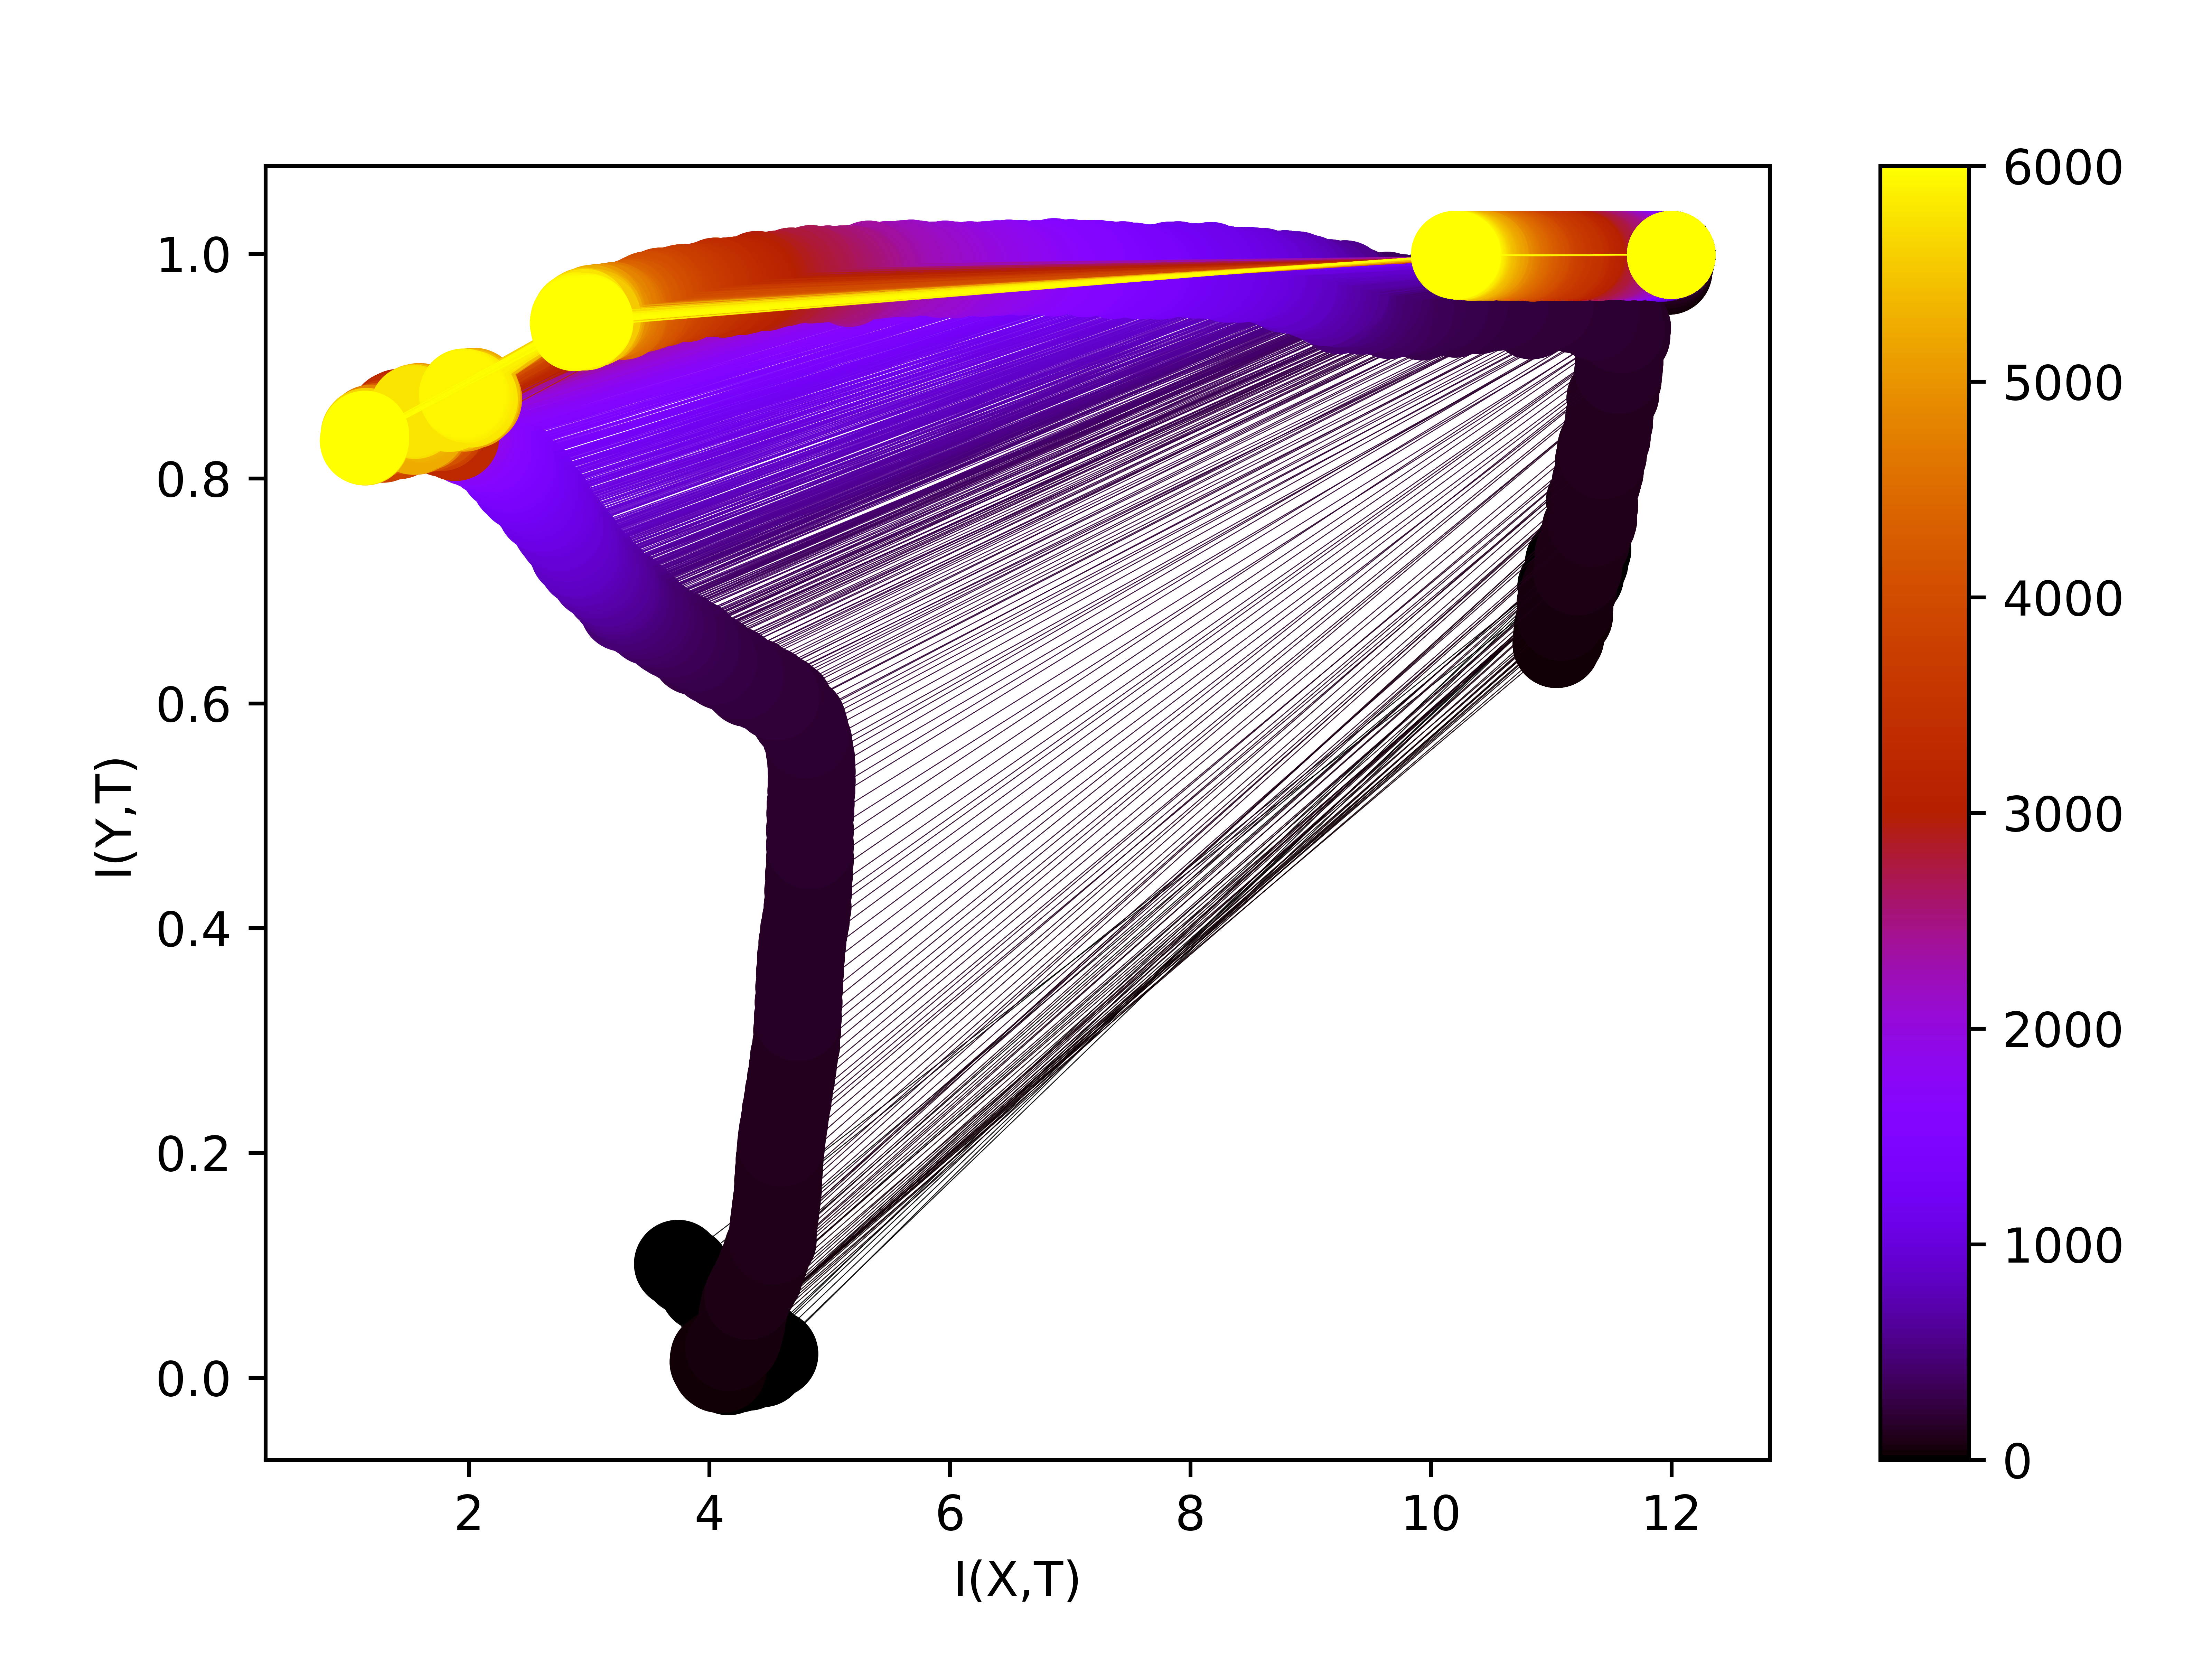
\includegraphics[width=\textwidth]{figs/eval/trainingSize/Binning40.png}
    \caption{
      Training size - 40\%
    }
    \label{figBinningTS40}
  \end{subfigure}
  \begin{subfigure}[t]{0.32\textwidth}
    \centering
    \includegraphics[width=\textwidth]{figs/eval/trainingSize/Binning70.png}
    \caption{
      Training size - 70\%
    }
    \label{figBinningTS70}
  \end{subfigure}
  \caption{
      Tweaking training size for Tishby's binning MIE.
    }
  \label{figTS}
\end{figure}

\begin{figure}[ht]
  \centering
  \begin{subfigure}[t]{0.32\textwidth}
    \centering
    \includegraphics[width=\textwidth]{figs/eval/networkShape/Binning10,4,2,2.png}
    \caption{
      Network Shape - 12,10,4,2,2,2
    }
    \label{figNetworkShapeDefault}
  \end{subfigure}
  \hfill
  \begin{subfigure}[t]{0.32\textwidth}
    \centering
    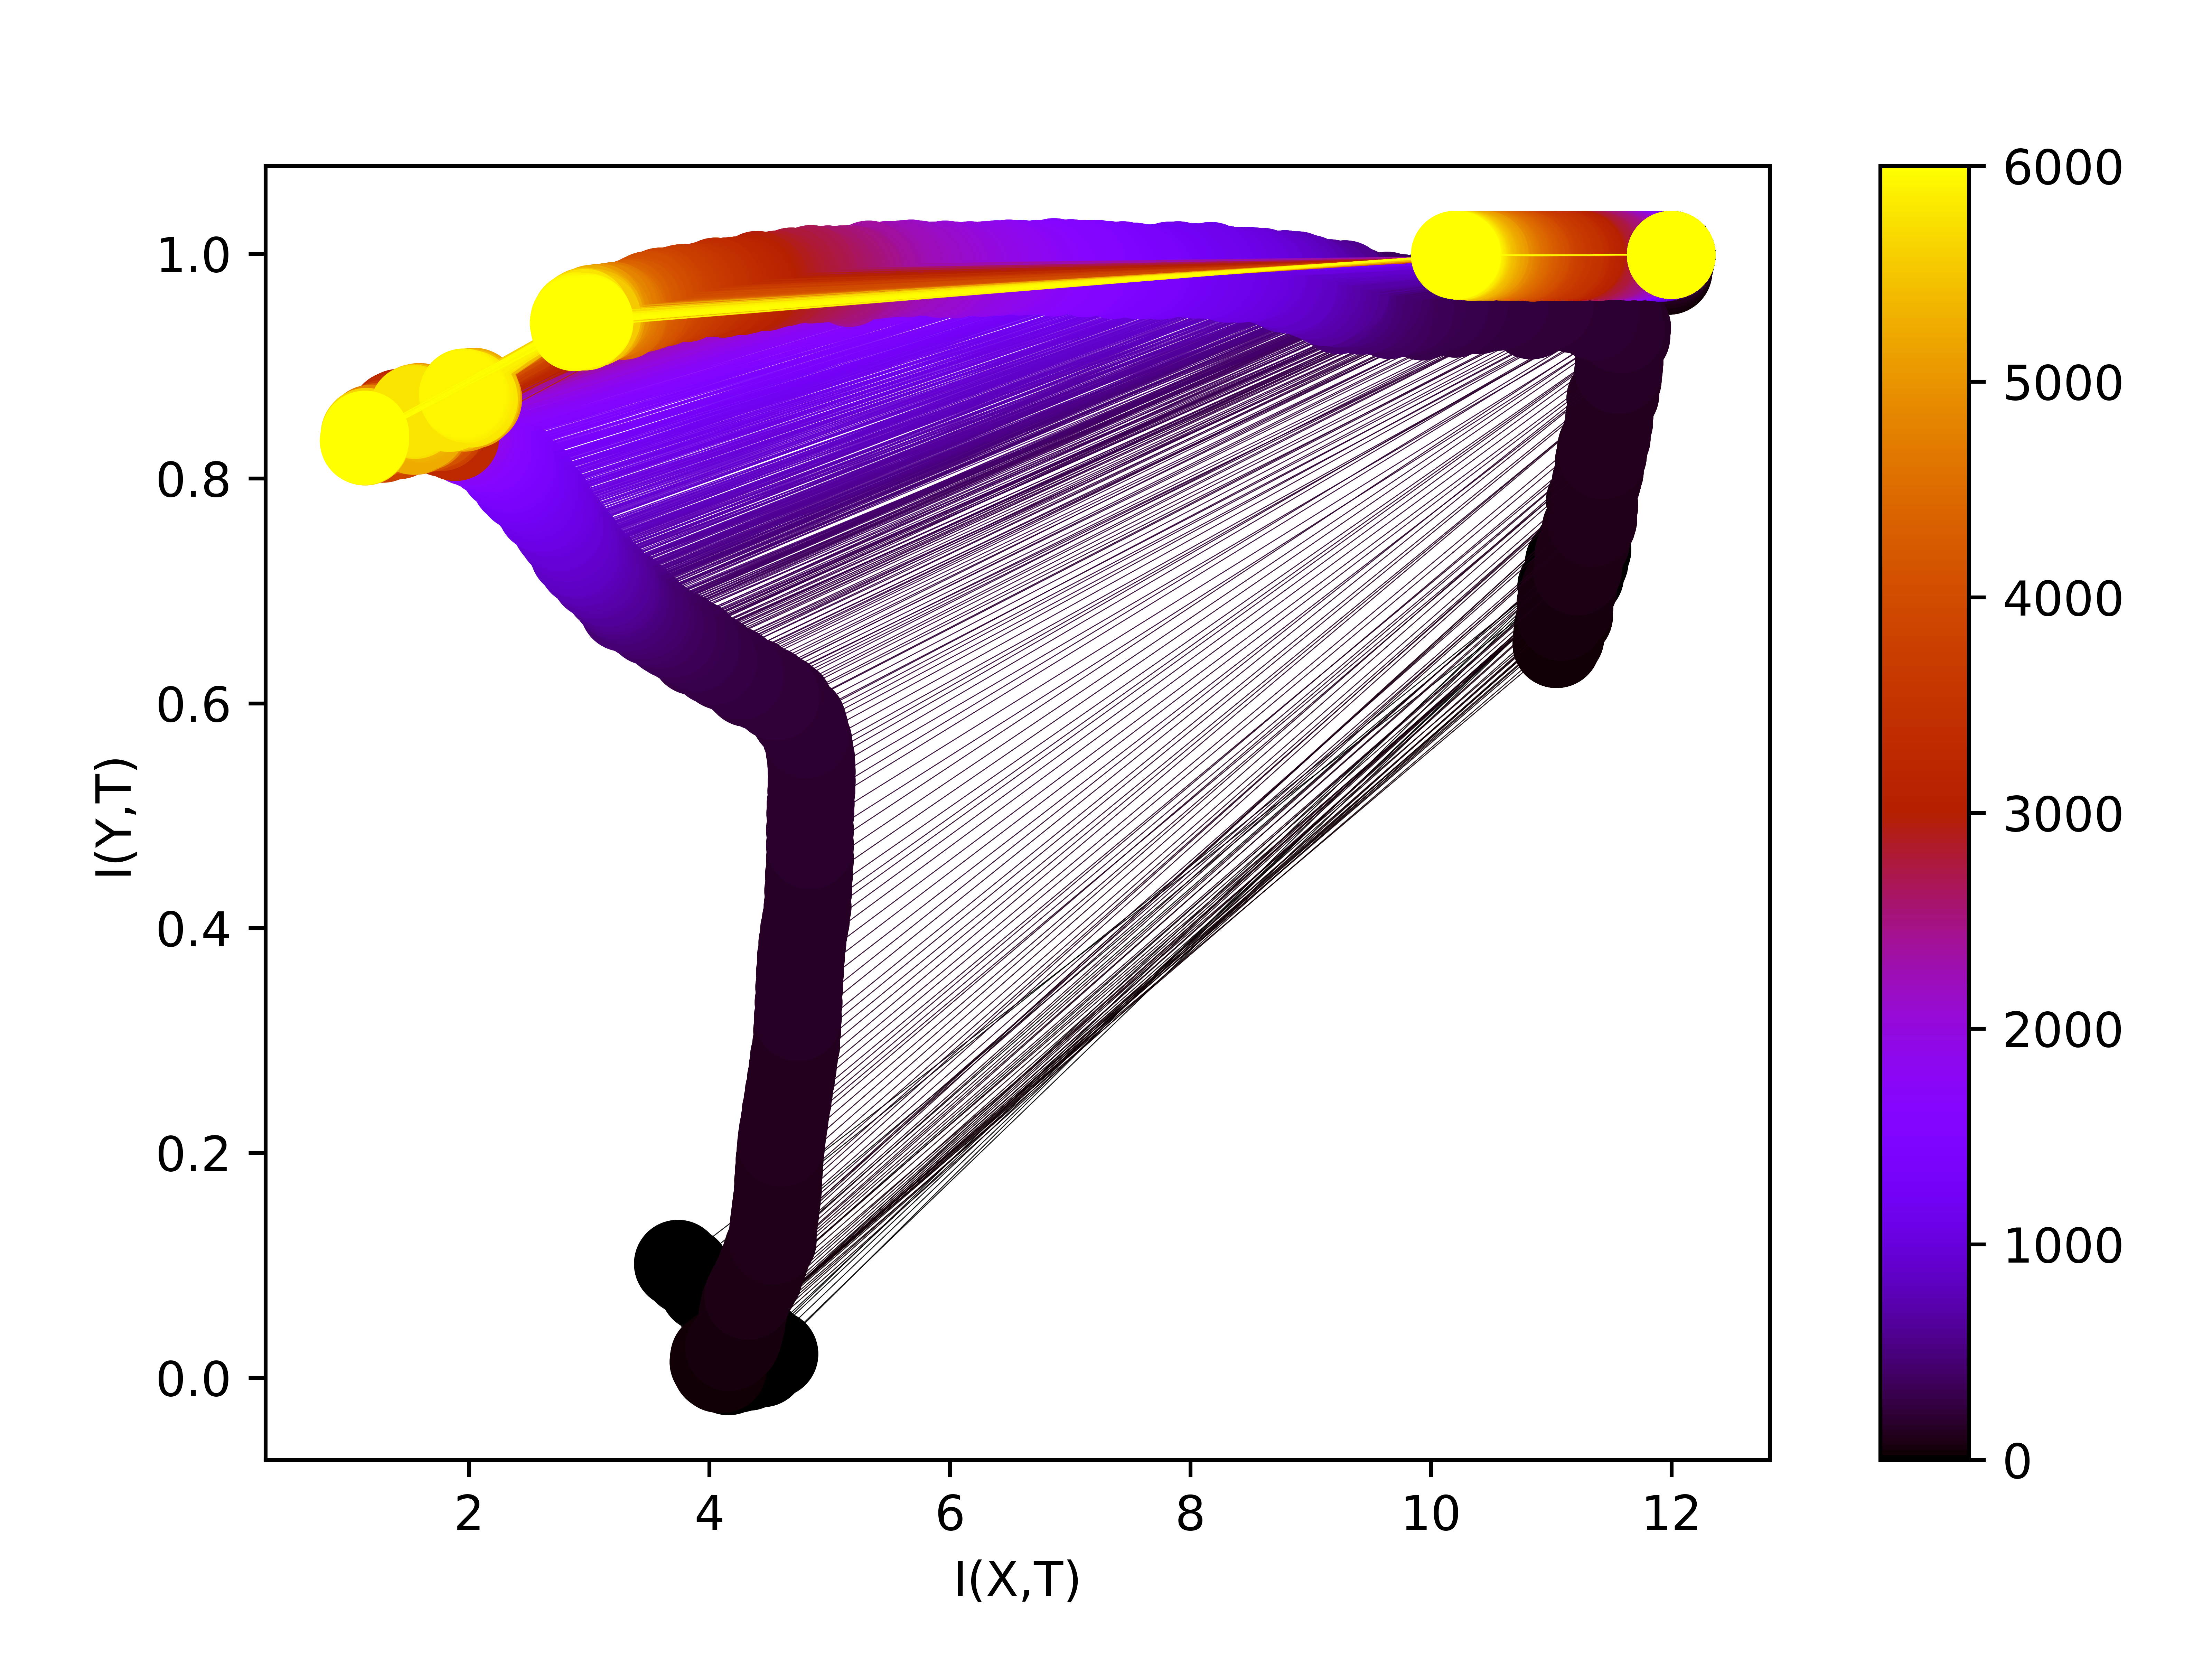
\includegraphics[width=\textwidth]{figs/eval/networkShape/Binning10,8,6,4.png}
    \caption{
      Network Shape - 12,10,8,6,4,2, Default
    }
    \label{figNetworkShape2}
  \end{subfigure}
  \hfill
  \begin{subfigure}[t]{0.32\textwidth}
    \centering
    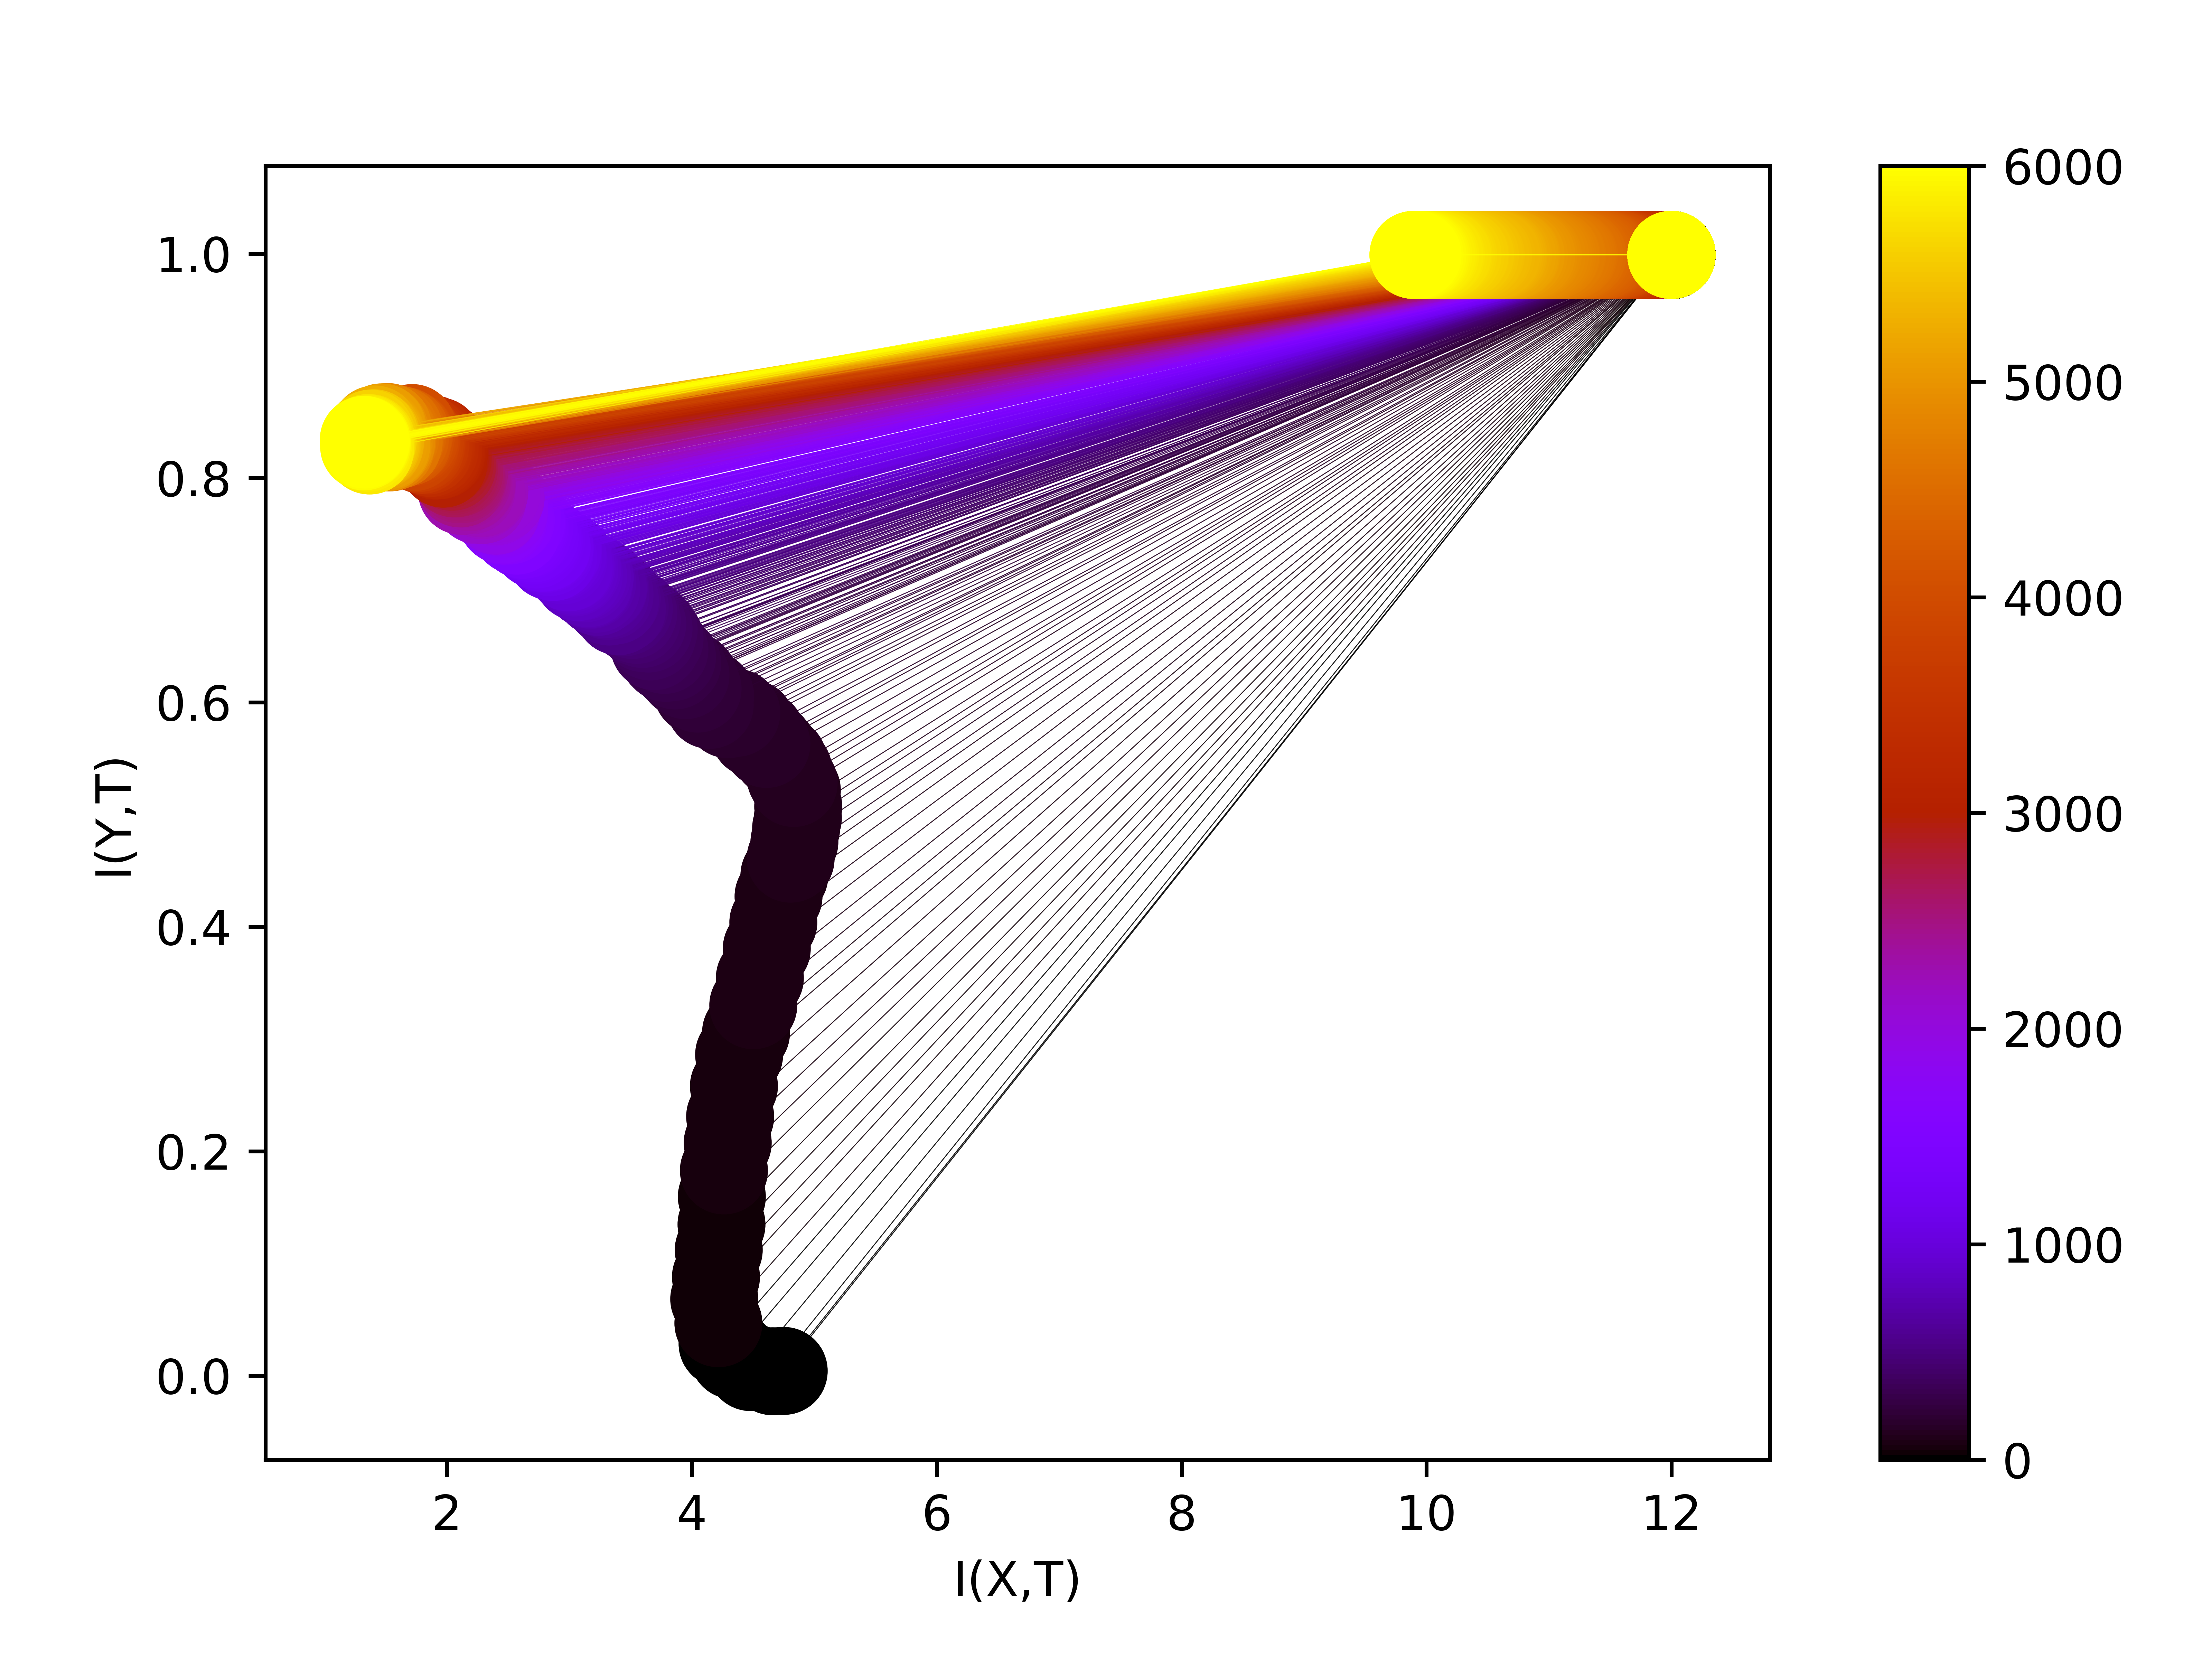
\includegraphics[width=\textwidth]{figs/eval/networkShape/Binning12,12,12.png}
    \caption{
      Network Shape - 12,12,12,12,2
    }
    \label{figNetworkShape3}
  \end{subfigure}
  \hfill
  \caption{
      Tweaking Network Shape for Tishby's binning MIE. 
    }
  \label{figNetworkShapes}
\end{figure}

\begin{figure}[ht]
  \begin{subfigure}[t]{0.3332\textwidth}
    \centering
    \includegraphics[width=\textwidth]{figs/eval/batchSize/Binning128.png}
    \caption{
      Batch size - 128
    }
    \label{figBatchSize128}
  \end{subfigure}
  \centering
  \begin{subfigure}[t]{0.3\textwidth}
    \centering
    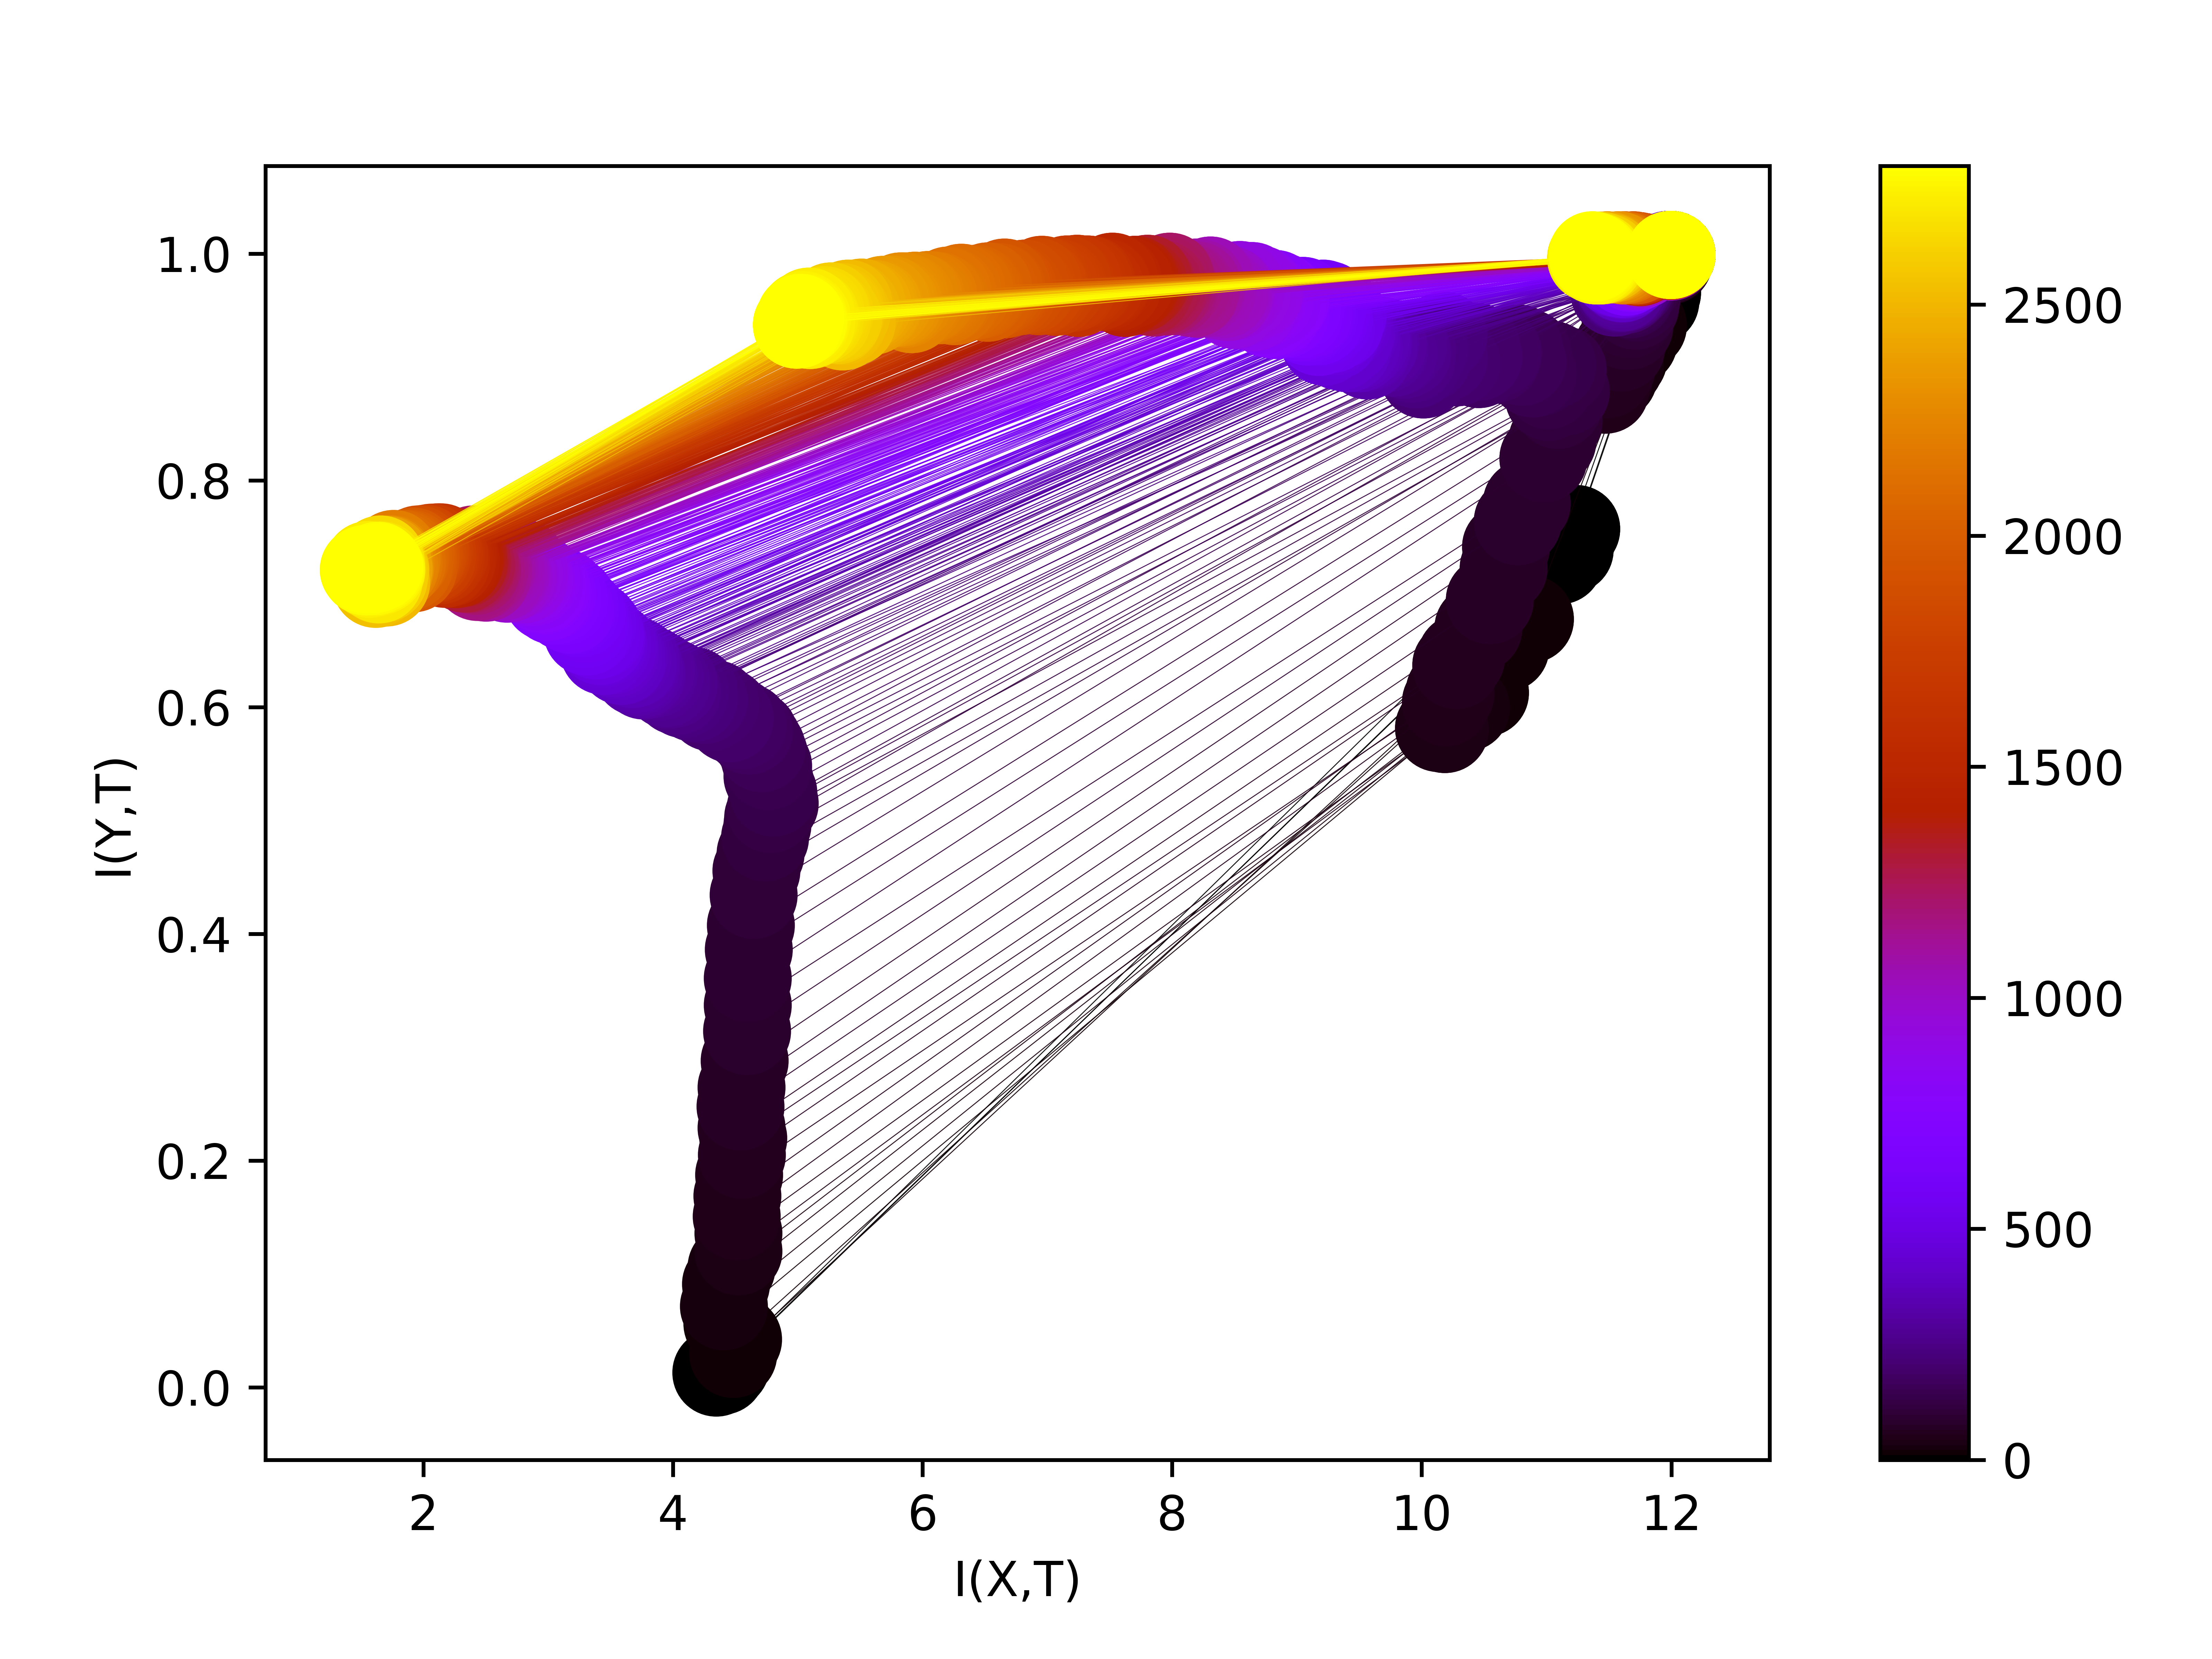
\includegraphics[width=\textwidth]{figs/eval/batchSize/Binning256.png}
    \caption{
      Batch size - 256
    }
    \label{figBatchSize256}
  \end{subfigure}
  \begin{subfigure}[t]{0.3332\textwidth}
    \centering
    \includegraphics[width=\textwidth]{figs/eval/batchSize/Binning512.png}
    \caption{
      Batch size - 512, Default
    }
    \label{figBatchSize512}
  \end{subfigure}
  \label{figBatchSize}
  \caption{
      Tweaking batch size for Tishby's binning MIE. Training Size - 20\%
    }
\end{figure}

\begin{figure}[ht]
  \centering
  \begin{subfigure}[t]{0.24\textwidth}
    \centering
    \includegraphics[width=\textwidth]{figs/eval/binCount/Binning10.png}
    \caption{
      Bin Count - 10
    }
    \label{figBinCount10}
  \end{subfigure}
  \hfill
  \begin{subfigure}[t]{0.24\textwidth}
    \centering
    \includegraphics[width=\textwidth]{figs/eval/binCount/Binning30.png}
    \caption{
      Bin Count - 30, Default
    }
    \label{figBinCount30}
  \end{subfigure}
  \hfill
  \begin{subfigure}[t]{0.24\textwidth}
    \centering
    \includegraphics[width=\textwidth]{figs/eval/binCount/Binning50.png}
    \caption{
      Bin Count - 50
    }
    \label{figBinCount50}
  \end{subfigure}
  \hfill
  \begin{subfigure}[t]{0.24\textwidth}
    \centering
    \includegraphics[width=\textwidth]{figs/eval/binCount/Binning80.png}
    \caption{
      Bin Count - 80
    }
    \label{figBinCount80}
  \end{subfigure}
  \hfill
  \caption{
      Tweaking bin count for Tishby's binning MIE. Training Size - 20\%
    }
  \label{figBinCount}
\end{figure}


\subparagraph{A note on activation functions} In every figure here the last
layer has the activation function $softmax$, so if we change the activation
function we should ignore the last layer as it might be misleading.

\subsection{Saxe's experiment} 

In his Paper Saxe claimed that Tishby's results are an epiphenomena of the
activation function $tanh$ and compression phase does not happen if we use the
ReLu activation function. Let us look at his experiments:
\begin{itemize}
  \item{
      The First one used the KDE as the MI estimator, and set the activation
      function to ReLu. All other values as default.
    }
  \item{
      And the second one used the KDE as the MI estimator, ReLu as the
      activation function, and MNIST as the dataset. All other values as default
    }
\end{itemize}
Notice that both of the experiments, changes MIE and the activation changes MIE
and the activation function at the same time. However, let us tweak the
hyperparameters independently:
\begin{itemize}
  \item{
      If we change activation function only, \autoref{figReluTanh}: The $\tanh$
      is as usual following the phases. However, The ReLu graph is completely
      different to the previous one. Every layer shows some signs of
      compression. However we cannot say that it supports Tishby's results.
      Having said that, it is also difficult to claim that compression phase
      does not happen for the activation function ReLu.
    }
  \item{
      If we change the MIE only, \autoref{figKDEBinning}: Notice:
      \begin{itemize}
        \item{
            If we only change the MIE we get completely different images.
            Leading to believe that one or both of the estimators are wrong.
          }
        \item{
            The figure produced by KDE MIE contradicts the Data Processing
            Inequality from \autoref{subsubPoMI} -- an impossible
            results.\footnote{It is possible I have made a mistake in my
            implementation, however the code for the KDE Entropy estimation is
            taken directly from the same code used for Saxe's paper.}
          }
      \end{itemize}
      
    }
\end{itemize}

\paragraph{A note on KDE}
When using the activation function $\tanh$ my
experiments consistently reproduced the impossible results. 
More precisely my experiments always showed a dip in information for the second
layer, then an increase for the consecutive layers. Which, seems to suggest the
estimator is broken.

However, if the activation function was ReLu the results seem to be in line with
what Saxe has presented in his paper. See Appendix \ref{appendixKDE}

\paragraph{} My results contradict the results produced by Saxe. 
However, there is suspicion that my implementation of KDE MIE is wrong -- so let
us discard the results from figure \autoref{figKDEBinKDE}.
Nevertheless, the results from figure \autoref{figReluTanhRelu}, suggest that
there might a \emph{compression phase} even if the activation function ReLu is
used.

\begin{figure}[ht]
  \centering
  \begin{subfigure}[t]{0.49\textwidth}
    \centering
    \includegraphics[width=0.7\textwidth]{figs/eval/activationFunction/BinningRelu.png}
    \caption{
      MIE - Binning, activation function - ReLu
    }
    \label{figReluTanhRelu}
  \end{subfigure}
  \begin{subfigure}[t]{0.49\textwidth}
    \centering
    \includegraphics[width=0.7\textwidth]{figs/eval/activationFunction/BinningTanh.png}
    \caption{
      MIE - Binning, activation function - $\tanh$
    }
    \label{figReluTanhTanh}
  \end{subfigure}
  \caption{
      Tweaking the activation function, ignore the last layer as it's
      activation function cannot be changed.
    }
  \label{figReluTanh}
\end{figure}


\begin{figure}[ht]
  \centering
  \begin{subfigure}[t]{0.49\textwidth}
    \centering
    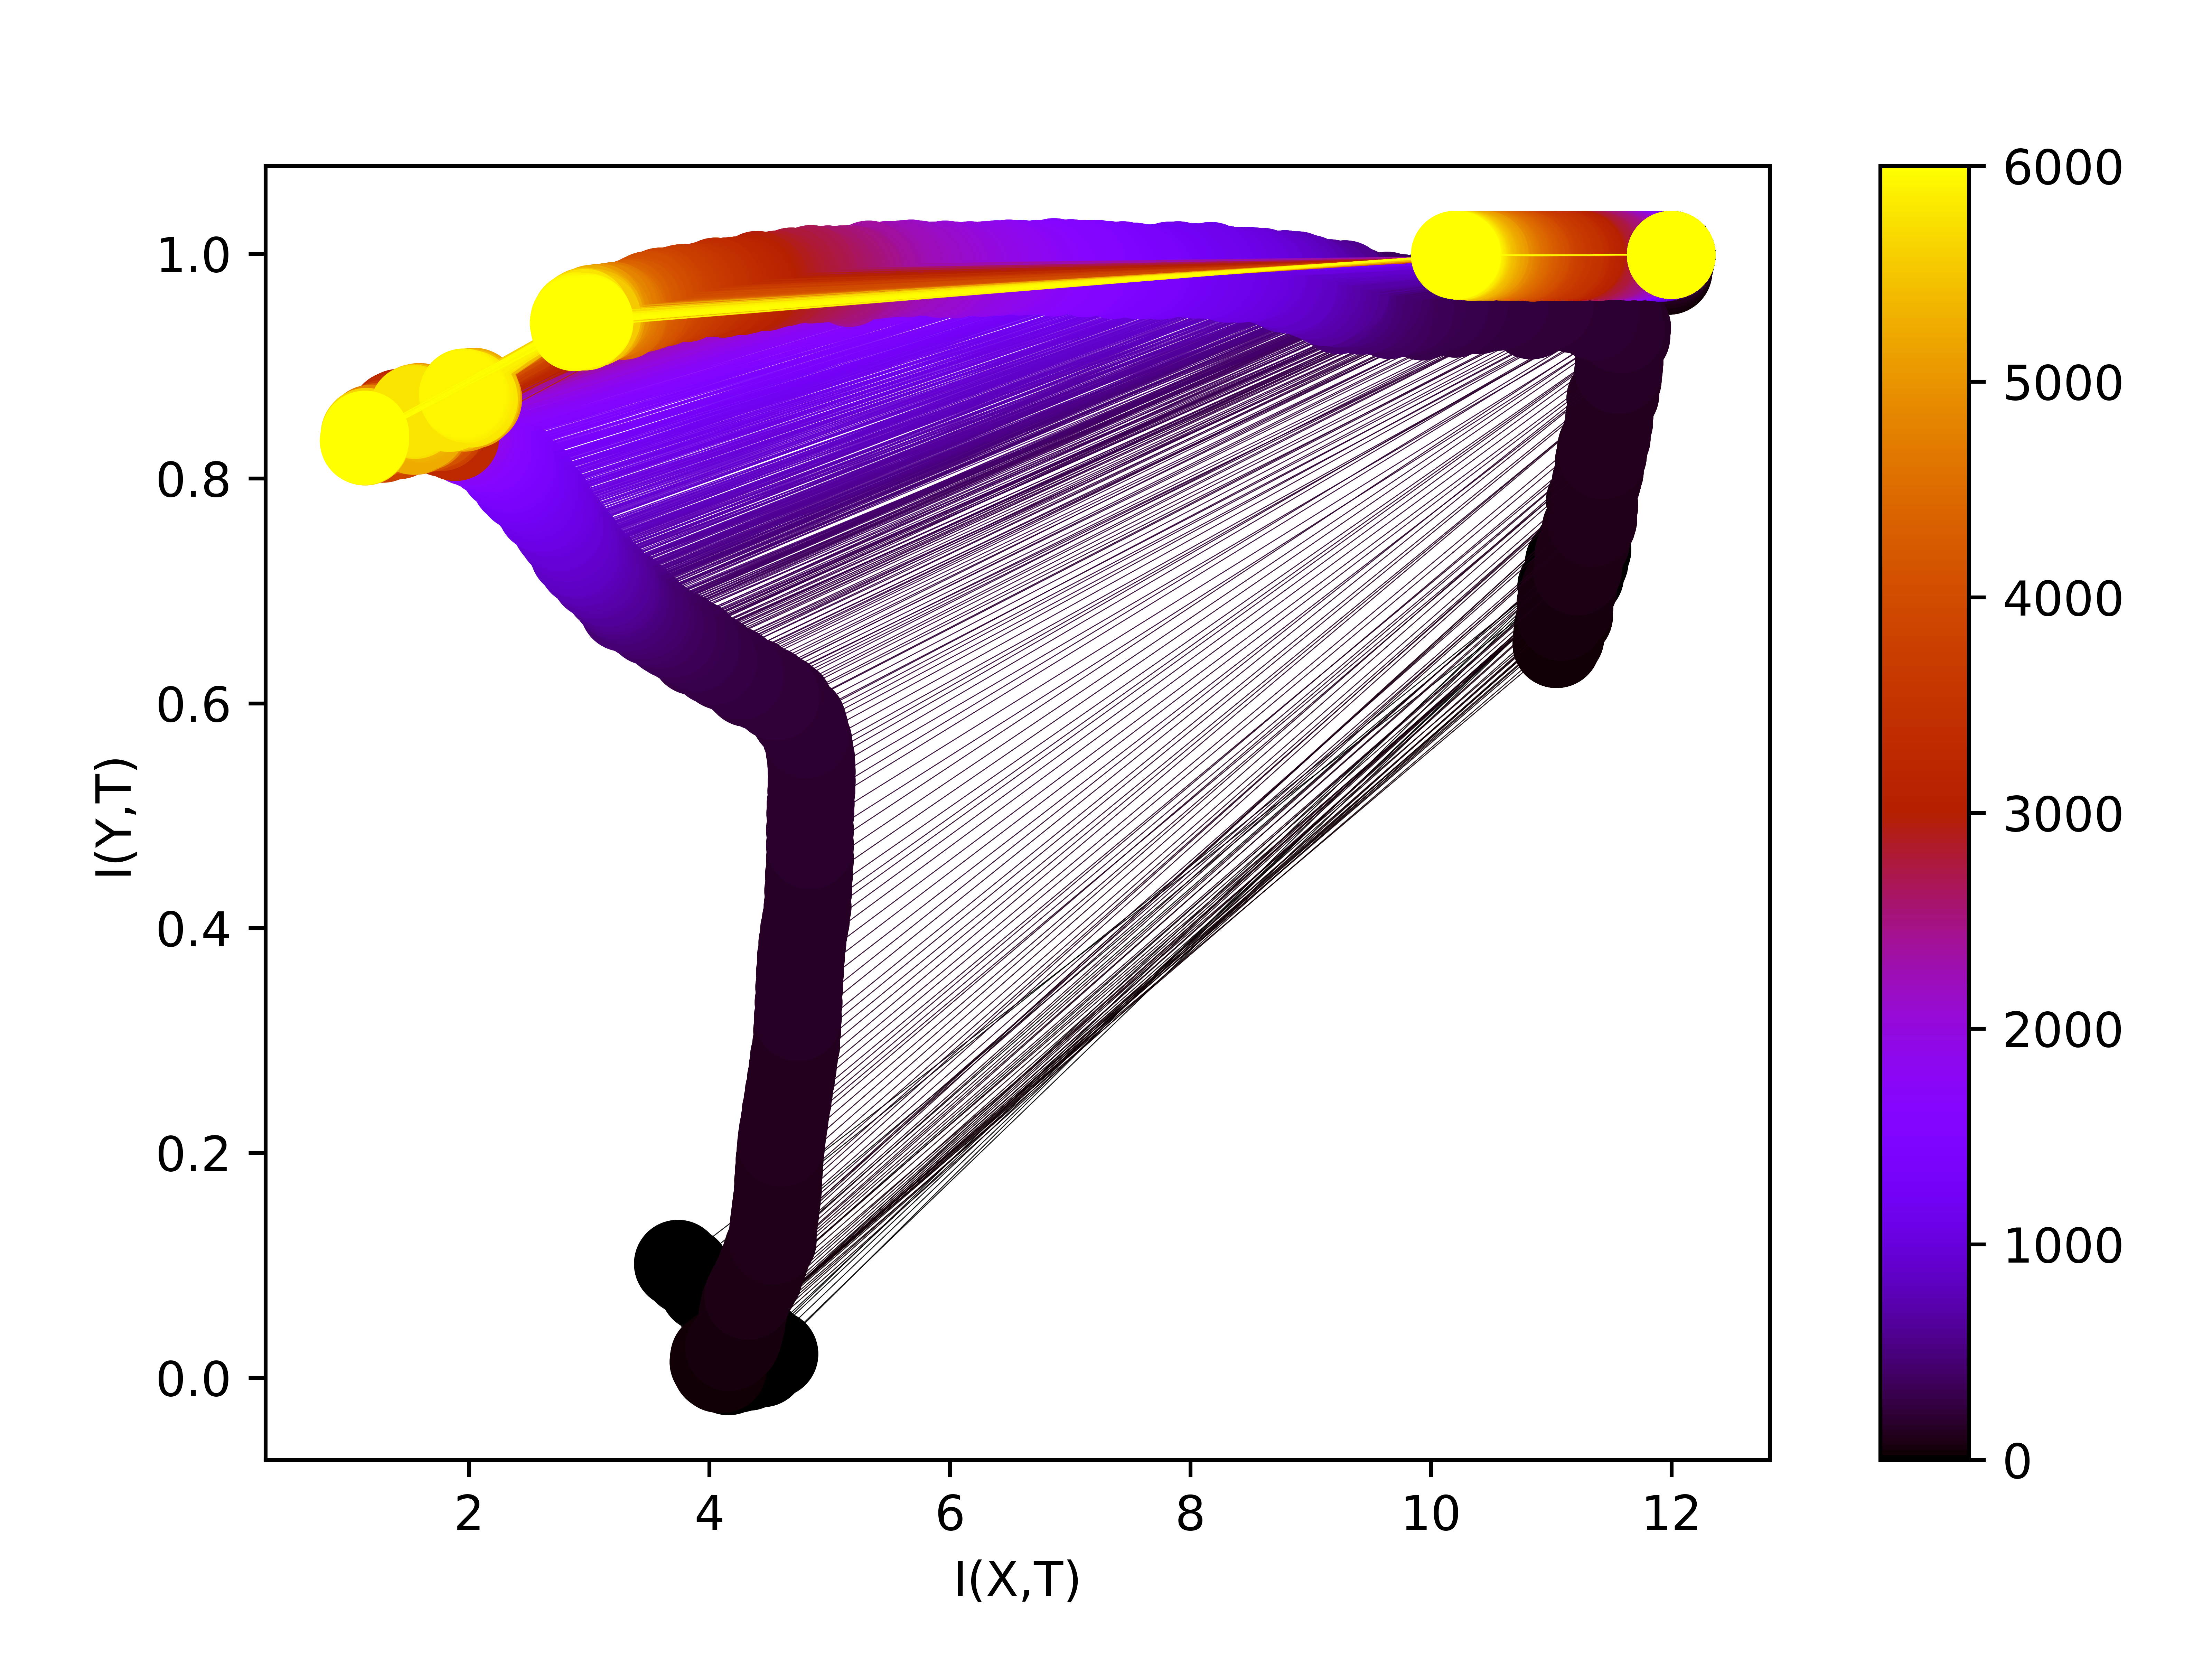
\includegraphics[width=0.7\textwidth]{figs/eval/trainingSize/Binning40.png}
    \caption{
      MIE - Binning, activation function - $\tanh$
    }
    \label{figKDEBinBin}
  \end{subfigure}
  \begin{subfigure}[t]{0.49\textwidth}
    \centering
    \includegraphics[width=0.7\textwidth]{figs/eval/trainingSize/KDE40.png}
    \caption{
      MIE - KDE, activation function - $\tanh$
    }
    \label{figKDEBinKDE}
  \end{subfigure}
  \caption{
      Tweaking the MIE.
    }
  \label{figKDEBinning}
\end{figure}

\section{Batching} 

Evaluating the Batching MIE is difficult.

\section{Ending remarks}
 
\begin{itemize}
  \item{
      Tishby and Saxe makes big claims about phases that a neural network is in
      NN. Such as "Is the compression phase an inherent part of NN and SGD
      algorithm" with out first agreeing on if compression can actually happen
      inside NNs.
    }
  \item{
      Furthermore, they are using very simple MIE.
    }
  \item{
      However they are using very simple MIE. In my opinion we need better tools
      before we can judge 
    }
\end{itemize}


\begin{itemize}
  \item{
      Success Criteria
    }
  \item{
      we have successfully reproduced the results showed by Tishby and Saxe.
      However there are reasons to not trust either of them as they have flaws
      with them.
      \begin{itemize}
        \item{
            Tishby -- used only a toy dataset 
          }
        \item{
            Saxe -- Changed allot of parameters at once made the claim that no
            compression phase happens
          }
      \end{itemize}
    }
  \item{
      We need better tools for MIE
      \begin{itemize}
        \item{
            cannot judge subtleties if something has a compression phase our MIE
            are not trustesd
          }
        \item{
            we have seen KDE and Discrete show inconsistent results, when n'th
            layers hass less information about the input than the n+1'th layer.
          }
      \end{itemize}
    }
  \item{
      compression phase 
      \begin{itemize}
        \item{
            judging if the networks have a compression phase is moot point as of
            yet as tools for measuring information are not good enough. Case and
            point Saxe argues that there cannot be compression in NN but every
            every experiments show that compression exists.
          }
        \item{
            Saxe states that there is no compression in NN, however their
            experiments disagree. 
          }
        \item{
            we don't have the tools to say if the compression phase is actually
            happening
          }
        \item{
            Tishby says compression phase happens but he is using a toy dataset,
            which was shown to not have a compression phase by Saxe.
          }
      \end{itemize}
    }
  \item{
      performance
    }
\end{itemize}


\end{document}
